\documentclass[12pt]{article}
\usepackage{epsfig,amsmath,amsthm,amssymb,amstext,vin}
\usepackage{amsthm,amsmath,amsfonts,amssymb,amscd,latexsym,txfonts}
\usepackage{mathrsfs,scalerel}
\usepackage{algpseudocode}
\usepackage{listings}
\usepackage{comment}
\usepackage{hyperref}
\usepackage{fancyhdr}
\usepackage{lastpage}

\textheight=8.5in
\textwidth=7in
\oddsidemargin=0.0in

\pagestyle{fancy}
\fancyhf{}
\rfoot{Page \thepage \hspace{1pt} of \pageref{LastPage}}

\newsavebox\foobox
\newlength{\foodim}
\newcommand{\slantbox}[2][0]{\mbox{%
        \sbox{\foobox}{#2}%
        \foodim=#1\wd\foobox
        \hskip \wd\foobox
        \hskip -0.5\foodim
        \pdfsave
        \pdfsetmatrix{1 0 #1 1}%
        \llap{\usebox{\foobox}}%
        \pdfrestore
        \hskip 0.5\foodim
}}
\def\Laplace{\ThisStyle{\slantbox[-.45]{$\SavedStyle\mathscr{L}$}}}

\begin{document}

\hbox{ % Horizontal box
\hspace*{0.2\textwidth} % Whitespace to the left of the title page
\rule{1pt}{\textheight} % Vertical line
\hspace*{0.05\textwidth} % Whitespace between the vertical line and title page text
\parbox[b]{0.75\textwidth}{ % Paragraph box which restricts text to less than the width of the page

{\noindent\Huge\bfseries Inverse Laplace transform and Post Inversion Formula}
\\[5\baselineskip] % Tagline or further description

{\large Student Investigator:  \Large \textsc{Qinmao Zhang}} % Author name
\\[1\baselineskip] % Tagline or further description
{\large Faculty Mentor: \textsc{ \Large Vincenzo Isaia}} % Author name
\\[6\baselineskip] % Tagline or further description

\vspace{0.23\textheight}

}}


\section{Introduction}

Laplace transform and inverse Laplace are powerful mathematical tools. Here is the definition of Laplace transform:
$$F(s) = \int_{0}^{\8} e^{-st} f(t) dt$$

To find Laplace or inverse Laplace transform, we usually substitutes with existing transform pairs. Many common problems can solved in this method, but not all functions in general. We are trying find a general approach that will work for any function.

For Laplace transform, its definition provides a good way to perform Laplace transform numerically. However, inverse Laplace transform is not as easy.
Fourier-integral is known to be identical to inverse Laplace transform. However, computing a complex contour integral numerically is nontrivial.
$$ \mathscr{L}^{-1}\{ F(s) \} = \frac{1}{2\pi i}\lim_{T \rightarrow \8} \int_{\lambda - i T}^{\lambda + i T} e^{s t} F(s) ds $$

This paper is dedicated to a research of general numerical approach to inverse Laplace transform based on Post Inversion Formula.
Post Inversion Formula, see for example \cite{KB}. is a theoretical equivalent to the inverse Laplace transform (See section 2 for more information). However, mathematicians often believe that it is too computational intensive to be put into practical usage. In this paper, however, we introduce an algorithm based on Parker–Sochacki method (PSM) (See section 3 for more information).
This paper also contains some example MATLAB codes and algorithm analysis.

All source codes are available in 
\href{https://github.com/fredzqm/laplace}{this gitHub repository}


\section{Post Inversion Formula Challenges}

Emil Post discovered Post's Inversion Formula, which is a simple-looking but usually impractical formula for evaluating an inverse Laplace transform. F(s) is the Laplace transform of f(t).
\begin{equation*}
f(t) = \lim_{k \rightarrow \8}\frac{(-1)^{k}}{k!} \left(\frac{k}{t}\right)^{k+1}  F^{(k)} \left(\frac{k}{t}\right)
\end{equation*}
As we can see from this formula, as k approaches infinity, we have several computational obstacles. 
\begin{enumerate}
\item
	\textbf{High order of derivatives}: As k approach infinity, $F^k(t)$ becomes an high order derivative. Traditionally, we approximate derivatives slopes between dense sample points, but the number of valid sample points drop half for an higher order derivative. If we want to have n sample points in k-th order derivative, we need $n*2^{k}$ sample points in the original function. As k grows, the traditional method has an intractable run-time.

\item 
	\textbf{Overflow and underflow}: $\frac{1}{k!}$ grows very tiny, while $\frac{k}{t}^{k+1}$ grows very large. Gigantic and tiny number are big challenges because double precision floating number ranges from $2.22507*10^{-308}$ to  $1.79769*10^{308}$. Those fast growing or diminishing number exceeds this range quickly. The experiment indicates overflow and underflow happen when k reaches around 180.
	Another source of overflow and underflow is high-order derivatives. For many functions, chain and product rules cause the derivatives to approach infinitesimal, quickly beyond the range of double precision floating number.

\item
 	\textbf{Slow convergence}: To acquire one single value, we need to perform a sequence of intensive computations to confirm the convergence. It is hard in general to know when it reaches the convergence and how accurate the result is. It is very inefficient to compute the formula above hundreds of time to get just one point in the final inverse Laplace transform curve.
\end{enumerate}

This paper will discuss the algorithm that solves the first two computational obstacles with PSM. The last obstacle is still troublesome. We are yet to develop smart program that carefully selects k value and claims convergence when error is small enough. In the end, we will show a few examples using Post Inversion Formula to perform inverse Laplace transform.

\section{Parker-–Sochacki method (PSM)}

This section will illustrate Parker-–Sochacki method and how it is used to calculate the high order derivatives, see \cite{OV}. PSM may sometimes also refers to Power Series method because it use high-order power series to approximate a certain function.

In brief, PSM produces the Taylor series of a function through Picard Iteration. Then, we can find the high order derivatives through those polynomials fairly quickly. Tradition method requires $O(n^{k})$ samples points, where k is the max derivative order. In contrast, PSM requires $O(k)$ iterations to reach an k-th order Taylor Series.

For instance, consider a three element differential equation system:
\begin{equation}
\frac{dx}{dt} = f_{x}(t, x, y, z) \qquad
\frac{dy}{dt} = f_{y}(t, x, y, z) \qquad
\frac{dz}{dt} = f_{z}(t, x, y, z)
\end{equation}	
\begin{equation}
x_{0}(t) = x_{0} \qquad
y_{0}(t) = y_{0} \qquad
z_{0}(t) = z_{0}
\end{equation}
We can use the following Picard Iteration formula to generate a sequence of $x_{n}(t),y_{n}(t),z_{n}(t)$. As n grows, those functions become closer to the solution of the differential system. See for example \cite{CL}
\begin{equation}
x_{n+1}(t) = x_{0} + \int_{t_{0}}^{t} f_{x}(t, x_{n}(t),y_{n}(t),z_{n}(t)) dt
\end{equation}
\begin{equation}
y_{n+1}(t) = y_{0} + \int_{t_{0}}^{t} f_{y}(t, x_{n}(t),y_{n}(t),z_{n}(t)) dt
\end{equation}
\begin{equation}
z_{n+1}(t) = z_{0} + \int_{t_{0}}^{t} f_{z}(t, x_{n}(t),y_{n}(t),z_{n}(t)) dt
\end{equation}
Picard iteration is popular numerical method to solve complex differential equation system. However, the system can only contain additions and multiplications arithmetic, referred as Normalized ODE in this paper.
Normalized system has a nice property. Since $x_{0}(t),y_{0}(t),z_{0}(t)$ are constants initially, their integrals $x_{n}(t),y_{n}(y),z_{n}(t)$ are all polynomials for the solution. Picard Iterative Process always generates Taylor approximations, see \cite{PS}. Computer program can also handle these simple arithmetic easily.


\subsection{Normalization of an arbitrary function}

Though Picard Iteration works for any kind of ODE, software can only handle normalized ODE. Therefore, all ODE need to be converted into the normalized form:
$$
y'(t) = \sum^N_{i=1} k_{i} t^{n_{1}} x^{a_{1}}(t) y^{b_{1}}(t) z^{c_{1}}(t) 
$$
$$
k_i \in \mathbb{R} \qquad n_i, a_i, b_i, c_i \in \mathbb{Z}^+_0
$$

There are vector fields that can not be normalized. Proof of existence of such a vector fields is given in \cite{CPSW}. However, because of the difficulty in constructing such a vector fields, the most vector fields in practice can be normalized by the following algorithm:
\begin{enumerate}
\item Check if all elements' derivative equations contain only additions and multiplications, we are done.
\item Find the biggest part in the equation containing arithmetic other than addition and multiplication, create an element to represent this part.
\item Find the derivative of the new element and replace all other matches in our system with it. Repeat step 1.
\end{enumerate}
For example, let's normalize the following vector field.
\begin{equation}
x(t) = \sqrt{t+1}\cos(t^2)  \qquad
x'(t) = \frac{\cos(t^2)}{2\sqrt{t+1}} - 2t\sqrt{t+1}*\sin(t^2)
\end{equation}
First of all, we see $2t\sqrt{t+1}*\sin(t^2)$ is the biggest part that involves a non-polynomial function, so create an element for that. 
\begin{equation}
y(t) = \sqrt{t+1}\sin(t^2)  \qquad
y'(t) = \frac{\sin(t^2)}{2\sqrt{t+1}} + 2t\sqrt{t+1}*\cos(t^2)
\end{equation}
Substitute as much as possible.
\begin{equation}
x(t) = \sqrt{t+1}\cos(t^2)  \qquad
x'(t) = \frac{x(t)}{2(t+1)} - 2t*y(t)
\end{equation}
\begin{equation}
y(t) = \sqrt{t+1}\sin(t^2)  \qquad
y'(t) = \frac{y(t)}{2(t+1)} + 2t*x(t)
\end{equation}
Create another element $z(t) = \frac{1}{t+1}$, and the final system turns out to be.
\begin{equation}
x'(t) = \frac{1}{2}x(t)*z(t) - 2t*y(t) \qquad
y'(t) = \frac{1}{2}y(t)*z(t) + 2t*x(t) \qquad
z'(t) = -z^{2}(t)
\end{equation}
This is a typical solution from the normalization algorithm. The organize format makes it easy for program to compute. We can now run Picard Iteration through this normalized system and get a Taylor approximation.

\subsection{Software Optimization}
Previous sections discussed the general idea of our approach, but to actual produce a feasible algorithm, the implementation needs to be optimized.

The MATLAB program developed takes an initial value problem (IVP).
It stores the results of Picard Iteration as an array. These arrays are initialized with initial value from IVP. Since all elements' derivatives are in normal forms, we can first compute products of polynomials with convolutions and add them up to produce the next iteration.

The convolution implementation in MATLAB looks something like:
\begin{algorithmic}
\For{\texttt{i = 1 to k}}
   \For{\texttt{j = 1 to k}}
      \State \texttt{c[i+j] += a[i] + b[j]]}
   \EndFor
\EndFor
\end{algorithmic}
However, as you can see, it takes $O(n^2)$, quite slow. Luckily, we can optimize this algorithm based on some nice features of Picard's Iterations for Normalized systems and eventually achieve linear run time.

\subsubsection{Settled Coefficients}

\noindent \textbf{Inductive hypothesis}:
In k-th iteration, any terms with order less than or equal to k are settled (remain the same value in later iteration).

\noindent \textbf{Base step}:
We know that 0-order terms are settled in iteration 0, since they are all constants from initial conditions.

\noindent \textbf{Inductive step}: 
In k-th iteration, any terms lower than $k^{th}$ are settled.
Notice integrating always produces a higher order term. Therefore, the $(k+1)^{th}$ order term is only affected by lower terms after integration. Therefore, in the next iteration, $k^{th}$ terms are also settled. 
\vspace{5mm}

From this proof, we can see that the first k terms of the results are settled in $k^{th}$ iteration, so there is no need for us to recompute those terms. The complete convolution also generate higher order terms than k+1, but these terms are subjected to changes in later iteration. Therefore, to avoid unnecessary computation, the program does not compute those terms either. As a result of discussion above, we write program to calculate convolution of $(k+1)^{th}$ order term only and appends only one more coefficient to each list. Therefore, each iteration use a quick convolution, an O(n) algorithm:

\begin{algorithmic}
\For{\texttt{i = 1 to k}}
   \State \texttt{c += a[i] + b[k-j]]}
\EndFor
\end{algorithmic}

\subsubsection{Save intermediate products}
When the normalized system has three or more elements multiplied together, the program needs to perform convolutions in steps. It needs to generate a complete coefficient list for the next convolution. The quick convolution algorithm can only be applied to the last one. For $a^{m}$, where $m>2$, the computation time goes back to $O((m-1)*n^2)$.
For instance, if we have high order normalized system.
\begin{equation}
a' = a^{15}
\end{equation}
At each iteration, the program has to perform 13 complete convolutions to get $a^{14}$ and one quick convolution to get the next term it needs. The total run time is $O(14n^{2}+n)$.

Quick convolution works for two element convolution because earlier values are stored. Those settled terms effectively save redundant computation. Therefore, we choose optimize this by breaking high order exponents down to many second order multiplication.

In the new version, elements are stored in {\it adders}, while intermediate products are stored in {\it multipliers}. In each iteration, each multiplier performs one quick convolution of two other units (either adders or multipliers), while each adder sum up terms with $kt^{n}$ from a other units. Each adder corresponds to one element in the system.

This design makes it possible for the same convolution to be saved and reused multiple times. For example, a two-element system: 
\begin{equation}
a' = - 2t^{2}*b^{2} + b
\end{equation}
\begin{equation}
b' = - 2t*b^{2}
\end{equation}
$b^{2}$ occurs twice. If the program does not store it as intermediate convolution result, this operation would be performed twice in every iteration. The adders and multipliers system not only reduce higher order system to $O(n^{2})$, but also effectively reduces many repeated calculations.

\subsubsection{Binary exponentiation}
Encountering high order exponentiation like $a^{15}$, we choose to apply binary exponentiation algorithm, which can calculate $a^{n}$ in O(ln(n)) time, see \cite{BE}. $a^{15}$ can be computed in the following sequence.
\begin{equation}
b = a * a;
c = b * b;
d = c * c;
e = d * c;
f = e * a;
a' = d * f;
\end{equation}

Many efforts were put into developing an algorithm to extract minimum number of cached intermediate products from an normalized ODE system. This algorithm (rephraseRel.m in the repos) tries to find common factor in each terms and aims to reduce the number of multiplication in the system. With the help of this script, the user can still input an normalized ODE, which will be automatically analyzed.


\section{Computational Problems}
Another big issue with implementing Post's Inversion Formula is the overflow and underflow problem. As part of the equation, $\frac{(-1)^{k}}{k!} (\frac{k}{t})^{k+1}$ involves number that grows exponentially. The limit in Post Inversion Formula eventually converges at a finite number because the big and tiny parts cancel each other. However, as k grows large, double precision numbers fail to capture its value.
If we want to use Post Inversion Formula, we have to figure out a way to represent large and tiny numbers without losing accuracy.

\subsubsection{Growing Derivatives}
For many common functions, its derivatives diminish as the order grows. 
In a few examples, $-\ln(F^{k}(s))$ is proportional to k. This grow rate poses great challenge to convolution calculation, where many products have to be summed.

One way we found to represent an extremely large or small number is with its logarithm. Any number can be represent with log of its absolute value and its sign.

The quick convolution algorithm involves two steps: multiply corresponding coefficients respectively and sum the products up. Multiplication becomes addition if numbers are represented as a logarithm. However, summation becomes quite tricky. To keep value bounded, the program cannot use exp() to recover the actual value.

This issue halted the research for a while, until the pattern of convolution was thoroughly studied. Among all the products being summed, many are much bigger than others ($10^{16}$ larger). Others are small enough to be ignored.
As for as the program is concerned, only a few large values contribute to the summation. 
The actual program in the end divides all products by the maximum among them, and then use exp() to recover from logarithm representation. This approach puts a cap on the largest value the program needs to handle. exp() converts tiny underflowing number to 0, since they are negligible. Those recovered numbers are summed and then convert back to logarithm representation for storage. Overflow problem is successfully handled.

Surprisingly, the logarithm storage method does not slow down the program but speeds it up. We make guesses a few possible causes:
\begin{enumerate}
\item Logarithm representation changes multiplications to additions. Multiplications are much slower than addition. Computing $e^{\ln(a)+\ln(b)}$ instead of $a b$ directly gain efficiency at the expense of some accuracy.
\item MATLAB well optimizes ln() and exp(), which take constant run time.
\item Most operations, including addition, ln(), exp() are performed as arrays, which are well optimized with parallel computing in MATLAB.
\end{enumerate}

\subsubsection{Constant Multifactor}

Another part of Post's Inversion Formula, $\frac{(-1)^{k}}{k!} (k)^{k+1}$ is only a function of k. This part can be calculated ahead of time to speed up the program. However, Factorial is a big challenge. Stirling approximation shows that $n!$ is around $\sqrt{2\pi n }(\frac{n}{e})^{n}$.
$$\ln(n!) = n*\ln(n) - n + O(\ln(n)) $$
However, an error of $O(ln(n))$ is not accurate enough for our purpose. 

A dynamic programming approach is used to accurately and efficiently calculate $\ln(n!)$. An array $a_{k}$ is defined as $a_{k} = ln(n!)$. Then we have the recurrence relationship -- $a_{k+1} = a_{k} + ln(n+1)$. This simple log-factorial array help the program to find constant part in constant time.


\section{Test MATLAB Codes}

In this section, we will discuss the interface of the developed software. The program can used in two ways.
\begin{enumerate}
\item Given an known function and its ODE, the program can perform inverse Laplace transform with Post's Inversion Formula.
\item Given an unknown differential equation system, the program use PSM method to approximate and plot its solution. The user can set the minimum interval between computation points and the minimum order of Taylor series for each point.
Then the program can use the estimated function values to perform inverse Laplace transform with Post's Inversion Formula.
\end{enumerate}
A few examples will shown to demonstrate the program.

\subsection{Interface for nornamlized differential equation system}

The first example is included to illustrate how to specify a normalized differential equation system, with the format of 
$$
y'(t) = \sum^N_{i=1} k_{i} t^{n_{1}} x^{a_{1}}(t) y^{b_{1}}(t) z^{c_{1}}(t) 
$$
$$
k_i \in \mathbb{R} \qquad n_i, a_i, b_i, c_i \in \mathbb{Z}^+_0
$$
Since each element's derivative can be expressed as the sum of a series of products, we decide to represent the system as a list of products. A struct rel() is defined for this purpose.
$$ \text{rel(addTo, coefficient , order, comps )}$$
First of all, for a system with n elements, each element in the system is given an id from 1 to n. The element with id 1 always represents the function we try to solve. Each product in the system is encoded in a rel struct.
\begin{enumerate}
\item "addTo" refers to the element this product will be added to;
\item "coefficient" refers to the constant coefficient;
\item "order" refers to the order of t in the system, 0 if no t needed; 
\item "comps" is a list of all the other elements multiplied.
\end{enumerate}

We will take a look at the complex function discussed in previous section.
This problem originates from section 3.1 of Warne's paper, see \cite{EX} for more details, which can cause trouble for many numerical methods.

\begin{equation}
x(t) = \sqrt{t+1}\cos(t^2)
\end{equation}
which is converted into the following normalized differential equation system.
\[
\left \{
  \begin{tabular}{ccc}
  $x'(t) = \frac{1}{2}x(t)*z(t) - 2t*y(t)$ \\
  $y'(t) = \frac{1}{2}y(t)*z(t) + 2t*x(t)$ \\
  $z'(t) = -z^{2}(t)$
  \end{tabular}
\right \}
\]
If we represent x, y, z with 1, 2 and 3 perspectively, we have following five products represented with rel();

\vspace{0.3cm}
\begin{tabular}{ccccc}
  $\frac{1}{2}x(t)*z(t)$  &  $- 2t*y(t)$ &
  $\frac{1}{2}y(t)*z(t)$ & $2t*x(t)$ & $-z^{2}(t)$ \\
  rel(1, 1/2, 0, [1 3]) & rel(1, -2 , 1 , [ 2 ] ) & 
  rel(2, 1/2, 0, [2 3]) & rel(2, 2 , 1 , [ 1 ] ) & rel(3, -1 , 0 , [3 3] )
\end{tabular}
\vspace{0.2cm}

A deterministic differential equation system also needs initial conditions at a start point. An array of numbers can represent the initial values of all elements in the system. If the result are already known, the user can also alternatively pass in a cell array of exact functions.
\begin{lstlisting}
s = simulator( { @(t)sqrt(t+1)*cos(t^2)  @(t)sqrt(t+1)*sin(t^2) ...
		 @(t)1/(t+1) } , 0 , ...
  	       [ rel(1,1/2, 0, [1 3]) rel(1,-2, 1, 2) ...
    		 rel(2,1/2, 0, [2 3]) rel(2, 2, 1, 1) ...
       		 rel(3, -1, 0, [3 3]) ] );
\end{lstlisting}

The simulator constructor takes three arguments -- the initial condition, start time and differential equation system represented with an array of rels.

\begin{lstlisting}
%% compute
% specifies the miminum order Taylor series (default:5)
s.minOrder = 10; 

% specifies the interval between each point (default:0.05).
s.minResetTime = 0.1; 

% launches the simulator and compute up to 20.
s.compute(20);

%% plot Taylor series
% specify the supposed answer to be compared with.
answer = @(x) sqrt(x+1).*cos(x.^2);
t = 0 :0.01: 10 ;
s.plot( t , answer );
\end{lstlisting}

\begin{figure}
\caption{Approximation curve from PSM}
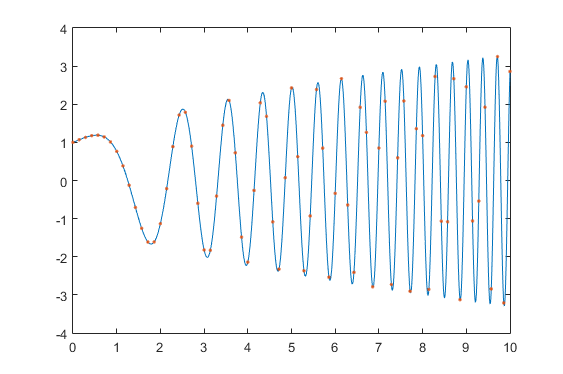
\includegraphics[scale=1]{nastyProb.png}
\end{figure}

After we have a simulator instance, the user can configure some parameters and ask the simulator to solve the system using PSM. The above codes use PSM method to calculate value from 0 to 20, and plot the result. As we can see, all the red dots (the correct answer) follow on the estimation (blue line). The PSM method successfully calculate the complex function.

\clearpage
\subsection{sin(t)}

\begin{equation}
\mathscr{L}^{-1}\{\frac{1}{s^2 + 1}\} = \sin(t) \quad\scriptscriptstyle
\end{equation}

The second example, we will illustrate how our program inverse Laplace transform. First of all, let's normalize the system and get the following simple form.
\begin{equation}
x(t) = \frac{1}{t^2 + 1} \quad x'(t) = \frac{2t}{(t^2 + 1)^2} = 2t *x(t)^2
\end{equation}
This system is then supplied into the system represented in the format illustrate in the previous section.
\begin{lstlisting}
s = simulator( {@(s)1/(s^2+1)} , 0 , ...
   [rel(1,-2, 1, [1 1]) ] );
   
%% convergence
figure(1)
hold off
t = 5;
kk = 1 : 100 : 1000;
answer = sin(t);
vv = s.converge( t , kk);
plot(kk , vv ,'-', kk , ones(1, size(kk,2)) * answer , '.');

%% inverseTransform
figure(4)
hold off
tt = 0 : 1 : 20;
k = @(t) t .^3 + 100;
answer = @(t) sin(t);
vv = s.converge( tt, ceil(k(tt)));
plot(tt, vv ,'-', tt, answer(tt), '.');

figure(5)
plot(tt, vv - answer(tt) ,'-');
\end{lstlisting}

s.converge(t, k) computes $v(t, k)$, given time and order. k needs to be large enough so the Post's Inversion formula converges.
If either or both of t and k is an array, an array of results will be returned.
\begin{equation*}
v(t, k) = \frac{(-1)^{k}}{k!} \left(\frac{k}{t}\right)^{k+1}  F^{(k)} \left(\frac{k}{t}\right)
\end{equation*}

The convergence section plots how v(t,k) converges to the inverse Laplace transform.

The inverseTransform section plots the actual Inverse Laplace transform. This example takes 17sec to compute.
The following table summarize the v(t,k), error and time to compute. As we can see, as t grows, it takes longer for v(t,k) to converge and needs larger k and longer time.

\begin{tabular}{| l | l | l | l | l | l |}
\hline
t  &  k   &  v(t,k) & sin(t) & error & time \\
\hline
1  &  100 &  0.8425 & 0.8415 & 0.001077 & 0.042 \\
\hline
1  &  1000 &  0.8416 & 0.8415 & 1.1838e-04 & 0.214 \\
\hline
1  &  10000 &  0.8415 & 0.8415 & 1.2057e-05 & 2.536 \\
\hline
10  &  100 &  -0.3622 & -0.5440 & 0.1819 & 0.070 \\
\hline
10  &  1000 &  -0.5252 & -0.5440 & 0.0189 & 0.209 \\
\hline
10  &  10000 &  -0.5421 & -0.5440 & 0.0019 & 2.566 \\
\hline
10  &  100000 &  -0.5438 & -0.5440 & 1.8907e-04 & 176.150\\
\hline
100  &  100 &  -4.4409e-16 & -0.5064 & 0.5064 & 0.072 \\
\hline
100  &  1000 &  -0.0047 & -0.5064 & 0.5016 & 0.072 \\
\hline
100  &  10000 &  -0.3036 & -0.5064 & 0.2027 & 2.673 \\
\hline
100  &  100000 &  -0.4809 & -0.5064 & 0.0255 & 148.276  \\
\hline
\end{tabular}

\clearpage
\begin{thebibliography}{99}
\bibitem{KB} Kurt Bryan. {\it Elementary Inversion of the Laplace Transform} https://www.rose-hulman.edu/~bryan/invlap.pdf

\bibitem{OV} G.E. Parker, J.S. Sochacki et al., An Overview of the Modied Picard
Method, http://educ.jmu.edu/sochacjs/expository.pdf

\bibitem{CL} E.A. Coddington and N. Levinson, Theory of Ordinary Differential Equations, McGraw-Hill, New York, 1955

\bibitem{PS} G.E. Parker and J.S. Sochacki, Implementing the Picard Iteration, Neural, Parallel and Scientic Computations, 4 (1996) 1, pp. 97-112.

\bibitem{CPSW} D.C. Carothers, G.E. Parker, J.S. Sochacki and P. G. Warne, Some
Properties of Solutions to Polynomial Systems of Equations, Elec. Jour. of Diff. Eqn.,
2005 (2005) 40, pp. 1-17.

\bibitem{EX} P. G. Warne, D. A. P. Warne, J. S. Sochacki, G. E. Parker and D. C.
Carothers, Explicit A-Priori Error Bounds and Adaptive Error Control for Approx-
imation of Nonlinear Initial Value Differential Systems, Comput. Math. Appl., 52
(2006), pp. 1695-1710.

\bibitem{PSM} Kurt Bryan. {\it Elementary Inversion of the Laplace Transform} https://www.rose-hulman.edu/~bryan/invlap.pdf

\bibitem{NORMAL} Kurt Bryan. {\it Elementary Inversion of the Laplace Transform} https://www.rose-hulman.edu/~bryan/invlap.pdf

\bibitem{SETTLE} Kurt Bryan. {\it Elementary Inversion of the Laplace Transform} https://www.rose-hulman.edu/~bryan/invlap.pdf

\bibitem{BE} Kurt Bryan. {\it Elementary Inversion of the Laplace Transform} https://www.rose-hulman.edu/~bryan/invlap.pdf

\end{thebibliography}

\end{document}